% Options for packages loaded elsewhere
\PassOptionsToPackage{unicode}{hyperref}
\PassOptionsToPackage{hyphens}{url}
\PassOptionsToPackage{dvipsnames,svgnames*,x11names*}{xcolor}
%
\documentclass[
]{article}
\usepackage{lmodern}
\usepackage{amssymb,amsmath}
\usepackage{ifxetex,ifluatex}
\ifnum 0\ifxetex 1\fi\ifluatex 1\fi=0 % if pdftex
  \usepackage[T1]{fontenc}
  \usepackage[utf8]{inputenc}
  \usepackage{textcomp} % provide euro and other symbols
\else % if luatex or xetex
  \usepackage{unicode-math}
  \defaultfontfeatures{Scale=MatchLowercase}
  \defaultfontfeatures[\rmfamily]{Ligatures=TeX,Scale=1}
  \setmainfont[]{cochineal}
  \setsansfont[]{Fira Sans}
  \setmonofont[]{Fira Code}
\fi
% Use upquote if available, for straight quotes in verbatim environments
\IfFileExists{upquote.sty}{\usepackage{upquote}}{}
\IfFileExists{microtype.sty}{% use microtype if available
  \usepackage[]{microtype}
  \UseMicrotypeSet[protrusion]{basicmath} % disable protrusion for tt fonts
}{}
\makeatletter
\@ifundefined{KOMAClassName}{% if non-KOMA class
  \IfFileExists{parskip.sty}{%
    \usepackage{parskip}
  }{% else
    \setlength{\parindent}{0pt}
    \setlength{\parskip}{6pt plus 2pt minus 1pt}}
}{% if KOMA class
  \KOMAoptions{parskip=half}}
\makeatother
\usepackage{xcolor}
\IfFileExists{xurl.sty}{\usepackage{xurl}}{} % add URL line breaks if available
\IfFileExists{bookmark.sty}{\usepackage{bookmark}}{\usepackage{hyperref}}
\hypersetup{
  pdftitle={Data Science for Economists},
  colorlinks=true,
  linkcolor=Maroon,
  filecolor=Maroon,
  citecolor=Blue,
  urlcolor=blue,
  pdfcreator={LaTeX via pandoc}}
\urlstyle{same} % disable monospaced font for URLs
\usepackage[margin=1in]{geometry}
\usepackage{color}
\usepackage{fancyvrb}
\newcommand{\VerbBar}{|}
\newcommand{\VERB}{\Verb[commandchars=\\\{\}]}
\DefineVerbatimEnvironment{Highlighting}{Verbatim}{commandchars=\\\{\}}
% Add ',fontsize=\small' for more characters per line
\usepackage{framed}
\definecolor{shadecolor}{RGB}{248,248,248}
\newenvironment{Shaded}{\begin{snugshade}}{\end{snugshade}}
\newcommand{\AlertTok}[1]{\textcolor[rgb]{0.94,0.16,0.16}{#1}}
\newcommand{\AnnotationTok}[1]{\textcolor[rgb]{0.56,0.35,0.01}{\textbf{\textit{#1}}}}
\newcommand{\AttributeTok}[1]{\textcolor[rgb]{0.13,0.29,0.53}{#1}}
\newcommand{\BaseNTok}[1]{\textcolor[rgb]{0.00,0.00,0.81}{#1}}
\newcommand{\BuiltInTok}[1]{#1}
\newcommand{\CharTok}[1]{\textcolor[rgb]{0.31,0.60,0.02}{#1}}
\newcommand{\CommentTok}[1]{\textcolor[rgb]{0.56,0.35,0.01}{\textit{#1}}}
\newcommand{\CommentVarTok}[1]{\textcolor[rgb]{0.56,0.35,0.01}{\textbf{\textit{#1}}}}
\newcommand{\ConstantTok}[1]{\textcolor[rgb]{0.56,0.35,0.01}{#1}}
\newcommand{\ControlFlowTok}[1]{\textcolor[rgb]{0.13,0.29,0.53}{\textbf{#1}}}
\newcommand{\DataTypeTok}[1]{\textcolor[rgb]{0.13,0.29,0.53}{#1}}
\newcommand{\DecValTok}[1]{\textcolor[rgb]{0.00,0.00,0.81}{#1}}
\newcommand{\DocumentationTok}[1]{\textcolor[rgb]{0.56,0.35,0.01}{\textbf{\textit{#1}}}}
\newcommand{\ErrorTok}[1]{\textcolor[rgb]{0.64,0.00,0.00}{\textbf{#1}}}
\newcommand{\ExtensionTok}[1]{#1}
\newcommand{\FloatTok}[1]{\textcolor[rgb]{0.00,0.00,0.81}{#1}}
\newcommand{\FunctionTok}[1]{\textcolor[rgb]{0.13,0.29,0.53}{\textbf{#1}}}
\newcommand{\ImportTok}[1]{#1}
\newcommand{\InformationTok}[1]{\textcolor[rgb]{0.56,0.35,0.01}{\textbf{\textit{#1}}}}
\newcommand{\KeywordTok}[1]{\textcolor[rgb]{0.13,0.29,0.53}{\textbf{#1}}}
\newcommand{\NormalTok}[1]{#1}
\newcommand{\OperatorTok}[1]{\textcolor[rgb]{0.81,0.36,0.00}{\textbf{#1}}}
\newcommand{\OtherTok}[1]{\textcolor[rgb]{0.56,0.35,0.01}{#1}}
\newcommand{\PreprocessorTok}[1]{\textcolor[rgb]{0.56,0.35,0.01}{\textit{#1}}}
\newcommand{\RegionMarkerTok}[1]{#1}
\newcommand{\SpecialCharTok}[1]{\textcolor[rgb]{0.81,0.36,0.00}{\textbf{#1}}}
\newcommand{\SpecialStringTok}[1]{\textcolor[rgb]{0.31,0.60,0.02}{#1}}
\newcommand{\StringTok}[1]{\textcolor[rgb]{0.31,0.60,0.02}{#1}}
\newcommand{\VariableTok}[1]{\textcolor[rgb]{0.00,0.00,0.00}{#1}}
\newcommand{\VerbatimStringTok}[1]{\textcolor[rgb]{0.31,0.60,0.02}{#1}}
\newcommand{\WarningTok}[1]{\textcolor[rgb]{0.56,0.35,0.01}{\textbf{\textit{#1}}}}
\usepackage{graphicx}
\makeatletter
\def\maxwidth{\ifdim\Gin@nat@width>\linewidth\linewidth\else\Gin@nat@width\fi}
\def\maxheight{\ifdim\Gin@nat@height>\textheight\textheight\else\Gin@nat@height\fi}
\makeatother
% Scale images if necessary, so that they will not overflow the page
% margins by default, and it is still possible to overwrite the defaults
% using explicit options in \includegraphics[width, height, ...]{}
\setkeys{Gin}{width=\maxwidth,height=\maxheight,keepaspectratio}
% Set default figure placement to htbp
\makeatletter
\def\fps@figure{htbp}
\makeatother
\setlength{\emergencystretch}{3em} % prevent overfull lines
\providecommand{\tightlist}{%
  \setlength{\itemsep}{0pt}\setlength{\parskip}{0pt}}
\setcounter{secnumdepth}{-\maxdimen} % remove section numbering
%% See: https://bookdown.org/yihui/rmarkdown-cookbook/multi-column.html
%% I've made some additional adjustments based on my own preferences (e.g. cols
%% should be top-aligned in case of uneven vertical length)
\newenvironment{columns}[1][]{}{}

\newenvironment{column}[1]{\begin{minipage}[t]{#1}\ignorespaces}{%
\end{minipage}
\ifhmode\unskip\fi
\aftergroup\useignorespacesandallpars
}

\def\useignorespacesandallpars#1\ignorespaces\fi{%
#1\fi\ignorespacesandallpars}

\makeatletter
\def\ignorespacesandallpars{%
  \@ifnextchar\par
    {\expandafter\ignorespacesandallpars\@gobble}%
    {}%
}
\makeatother

\title{Data Science for Economists}
\usepackage{etoolbox}
\makeatletter
\providecommand{\subtitle}[1]{% add subtitle to \maketitle
  \apptocmd{\@title}{\par {\large #1 \par}}{}{}
}
\makeatother
\subtitle{Lecture 7: Webscraping: (2) Client-side and APIs}
\usepackage{authblk}
                                        \author[]{Grant R. McDermott}
                                                            \affil{University
of Oregon \textbar{} \href{https://github.com/uo-ec607/lectures}{EC
607}}
                                            \date{}

\begin{document}
\maketitle

{
\hypersetup{linkcolor=}
\setcounter{tocdepth}{2}
\tableofcontents
}
\hypertarget{sign-up-and-software-requirements}{%
\subsection{Sign-up and software
requirements}\label{sign-up-and-software-requirements}}

\hypertarget{sign-up}{%
\subsubsection{Sign-up}\label{sign-up}}

We're going to be downloading economic data from the FRED API. This will
require that you first
\href{https://research.stlouisfed.org/useraccount/apikey}{create a user
account} and then
\href{https://research.stlouisfed.org/useraccount/apikey}{register a
personal API key}.

\hypertarget{external-software}{%
\subsubsection{External software}\label{external-software}}

Today I'll be using \href{https://jsonview.com/}{JSONView}, a browser
extension that renders JSON output nicely in Chrome and Firefox. (Not
required, but recommended.)

\hypertarget{r-packages}{%
\subsubsection{R packages}\label{r-packages}}

\begin{itemize}
\tightlist
\item
  New: \textbf{jsonlite}, \textbf{httr}, \textbf{listviewer},
  \textbf{usethis}, \textbf{fredr}
\item
  Already used: \textbf{tidyverse}, \textbf{lubridate},
  \textbf{hrbrthemes}, \textbf{janitor}
\end{itemize}

Here's a convenient way to install (if necessary) and load all of the
above packages.

\begin{Shaded}
\begin{Highlighting}[]
\DocumentationTok{\#\# Load and install the packages that we\textquotesingle{}ll be using today}
\ControlFlowTok{if}\NormalTok{ (}\SpecialCharTok{!}\FunctionTok{require}\NormalTok{(}\StringTok{"pacman"}\NormalTok{)) }\FunctionTok{install.packages}\NormalTok{(}\StringTok{"pacman"}\NormalTok{)}
\NormalTok{pacman}\SpecialCharTok{::}\FunctionTok{p\_load}\NormalTok{(tidyverse, httr, lubridate, hrbrthemes, janitor, jsonlite, fredr, }
\NormalTok{               listviewer, usethis)}
\DocumentationTok{\#\# My preferred ggplot2 plotting theme (optional)}
\FunctionTok{theme\_set}\NormalTok{(hrbrthemes}\SpecialCharTok{::}\FunctionTok{theme\_ipsum}\NormalTok{())}
\end{Highlighting}
\end{Shaded}

\hypertarget{recap-from-last-time}{%
\subsection{Recap from last time}\label{recap-from-last-time}}

During the last lecture, we saw that websites and web applications fall
into two categories: 1) Server-side and 2) Client-side. We then
practiced scraping data that falls into the first category ---
i.e.~rendered server-side --- using the \textbf{rvest} package. This
technique focuses on CSS selectors (with help from
\href{http://selectorgadget.com/}{SelectorGadget}) and HTML tags. We
also saw that webscraping often involves as much art as science. The
plethora of CSS options and the flexibility of HTML itself means that
steps which work perfectly well on one website can easily fail on
another website.

Today we focus on the second category: Scraping web data that is
rendered \textbf{client-side}. The good news is that, when available,
this approach typically makes it much easier to scrape data from the
web. The downside is that, again, it can involve as much art as it does
science. Moreover, as I emphasised last time, just because because we
\emph{can} scrape data, doesn't mean that we \emph{should}
(i.e.~ethical, legal and other considerations). These admonishments
aside, let's proceed\ldots{}

\hypertarget{client-side-apis-and-api-endpoints}{%
\subsection{Client-side, APIs, and API
endpoints}\label{client-side-apis-and-api-endpoints}}

Recall that websites or applications that are built using a
\textbf{client-side} framework typically involve something like the
following steps:

\begin{itemize}
\tightlist
\item
  You visit a URL that contains a template of static content (HTML
  tables, CSS, etc.). This template itself doesn't contain any data.
\item
  However, in the process of opening the URL, your browser sends a
  \emph{request} to the host server.
\item
  If your request if valid, then the server issues a \emph{response}
  that fetches the necessary data for you and renders the page
  dynamically in your browser.
\item
  The page that you actually see in your browser is thus a mix of static
  content and dynamic information that is rendered by your browser
  (i.e.~the ``client'').
\end{itemize}

All of this requesting, responding and rendering takes places through
the host application's \textbf{API} (or \textbf{A}pplication
\textbf{P}rogram \textbf{I}nterface). Time for a student presentation to
go over APIs in more depth\ldots{}

\hypertarget{student-presentation-apis}{%
\subsubsection{Student presentation:
APIs}\label{student-presentation-apis}}

If you're new to APIs or reading this after the fact, then I recommend
this excellent resource from Zapier:
\href{https://zapier.com/learn/apis/}{An Introduction to APIs}. It's
fairly in-depth, but you don't need to work through the whole thing to
get the gist. The summary version is that an API is really just a
collection of rules and methods that allow different software
applications to interact and share information. This includes not only
web servers and browsers, but also software packages like the R
libraries we've been using.\footnote{Fun fact: A number of R packages
  that we'll be using later in this course (e.g.~\textbf{leaflet},
  \textbf{plotly}, etc.) are really just a set of wrapper functions that
  interact with the underlying APIs and convert your R code into some
  other language (e.g.~JavaScript).} Key concepts include:

\begin{itemize}
\tightlist
\item
  \textbf{Server:} A powerful computer that runs an API.
\item
  \textbf{Client:} A program that exchanges data with a server through
  an API.
\item
  \textbf{Protocol:} The ``etiquette'' underlying how computers talk to
  each other (e.g.~HTTP).
\item
  \textbf{Methods:} The ``verbs'' that clients use to talk with a
  server. The main one that we'll be using is \texttt{GET} (i.e.~ask a
  server to retrieve information), but other common methods are
  \texttt{POST}, \texttt{PUT} and \texttt{DELETE}.
\item
  \textbf{Requests:} What the client asks of the server (see Methods
  above).
\item
  \textbf{Response:} The server's response. This includes a \emph{Status
  Code} (e.g.~``404'' if not found, or ``200'' if successful), a
  \emph{Header} (i.e.~meta-information about the reponse), and a
  \emph{Body} (i.e the actual content that we're interested in).
\item
  Etc.
\end{itemize}

\hypertarget{a-bit-more-about-api-endpoints}{%
\subsubsection{A bit more about API
endpoints}\label{a-bit-more-about-api-endpoints}}

A key point in all of this is that, in the case of web APIs, we can
access information \emph{directly} from the API database if we can
specify the correct URL(s). These URLs are known as an \textbf{API
endpoints}.

API endpoints are in many ways similar to the normal website URLs that
we're all used to visiting. For starters, you can navigate to them in
your web browser. However, whereas normal websites display information
in rich HTML content --- pictures, cat videos, nice formatting, etc. ---
an API endpoint is much less visually appealing. Navigate your browser
to an API endpoint and you'll just see a load of seemingly unformatted
text. In truth, what you're really seeing is (probably) either
\href{https://en.wikipedia.org/wiki/JSON}{JSON}
(\textbf{J}ava\textbf{S}cript \textbf{O}bject \textbf{No}tation) or
\href{https://en.wikipedia.org/wiki/XML}{XML} (E\textbf{x}tensible
\textbf{M}arkup \textbf{L}anguage).

You don't need to worry too much about the syntax of JSON and XML. The
important thing is that the object in your browser --- that load of
seemingly unformatted text --- is actually very precisely structured and
formatted. Moreover, it contains valuable information that we can easily
read into R (or Python, Julia, etc.) We just need to know the right API
endpoint for the data that we want.

Let's practice doing this through a few example applications. I'll start
with the simplest case (no API key required, explicit API endpoint) and
then work through some more complicated examples.

\hypertarget{application-1-trees-of-new-york-city}{%
\subsection{Application 1: Trees of New York
City}\label{application-1-trees-of-new-york-city}}

\href{https://opendata.cityofnewyork.us/}{NYC Open Data} is a pretty
amazing initiative. Its mission is to ``make the wealth of public data
generated by various New York City agencies and other City organizations
available for public use''. You can get data on everything from arrest
data, to the location of wi-fi hotspots, to city job postings, to
homeless population counts, to dog licenses, to a directory of toilets
in public parks\ldots{} The list goes on. I highly encourage you to
explore in your own time, but we're going to do something ``earthy'' for
this first application: Download a sample of tree data from the
\href{https://data.cityofnewyork.us/Environment/2015-Street-Tree-Census-Tree-Data/uvpi-gqnh}{\textbf{2015
NYC Street Tree Census}}.

I wanted to begin with an example from NYC Open Data, because you don't
need to set up an API key in advance.\footnote{Truth be told: To avoid
  rate limits --- i.e.~throttling the number of requests that you can
  make per hour --- it's best to
  \href{https://data.cityofnewyork.us/profile/app_tokens}{sign up} for
  an NYC Open Data app token. We're only going to make one or two
  requests here, though so we should be fine.} All you need to do is
complete the following steps:

\begin{itemize}
\tightlist
\item
  Open the
  \href{https://data.cityofnewyork.us/Environment/2015-Street-Tree-Census-Tree-Data/uvpi-gqnh}{web
  page} in your browser (if you haven't already done so).
\item
  You should immediately see the \textbf{API} tab. Click on it.
\item
  Copy the
  \href{https://data.cityofnewyork.us/resource/nwxe-4ae8.json}{API
  endpoint} that appears in the popup box.
\item
  \emph{Optional:} Paste that endpoint into a new tab in your browser.
  You'll see a bunch of JSON text, which you can render nicely using the
  JSONView browser extension that we installed earlier.
\end{itemize}

Here's a GIF of me completing these steps:

\begin{verbatim}
## Sorry, this GIF is only available in the the HTML version of the notes.
\end{verbatim}

Now that we've located the API endpoint, let's read the data into R.
We'll do so using the \texttt{fromJSON()} function from the excellent
\textbf{jsonlite} package
(\href{https://cran.r-project.org/web/packages/jsonlite/index.html}{link}).
This will automatically coerce the JSON array into a regular R data
frame. However, I'll go that little bit further and convert it into a
tibble, since the output is nicer to work with.

\begin{Shaded}
\begin{Highlighting}[]
\CommentTok{\# library(jsonlite) \#\# Already loaded}

\NormalTok{nyc\_trees }\OtherTok{=} 
  \FunctionTok{fromJSON}\NormalTok{(}\StringTok{"https://data.cityofnewyork.us/resource/nwxe{-}4ae8.json"}\NormalTok{) }\SpecialCharTok{\%\textgreater{}\%}
  \FunctionTok{as\_tibble}\NormalTok{()}
\NormalTok{nyc\_trees}
\end{Highlighting}
\end{Shaded}

\begin{verbatim}
## # A tibble: 1,000 x 45
##    tree_id block~1 creat~2 tree_~3 stump~4 curb_~5 status health spc_l~6 spc_c~7
##    <chr>   <chr>   <chr>   <chr>   <chr>   <chr>   <chr>  <chr>  <chr>   <chr>  
##  1 180683  348711  2015-0~ 3       0       OnCurb  Alive  Fair   Acer r~ red ma~
##  2 200540  315986  2015-0~ 21      0       OnCurb  Alive  Fair   Quercu~ pin oak
##  3 204026  218365  2015-0~ 3       0       OnCurb  Alive  Good   Gledit~ honeyl~
##  4 204337  217969  2015-0~ 10      0       OnCurb  Alive  Good   Gledit~ honeyl~
##  5 189565  223043  2015-0~ 21      0       OnCurb  Alive  Good   Tilia ~ Americ~
##  6 190422  106099  2015-0~ 11      0       OnCurb  Alive  Good   Gledit~ honeyl~
##  7 190426  106099  2015-0~ 11      0       OnCurb  Alive  Good   Gledit~ honeyl~
##  8 208649  103940  2015-0~ 9       0       OnCurb  Alive  Good   Tilia ~ Americ~
##  9 209610  407443  2015-0~ 6       0       OnCurb  Alive  Good   Gledit~ honeyl~
## 10 192755  207508  2015-0~ 21      0       Offset~ Alive  Fair   Platan~ London~
## # ... with 990 more rows, 35 more variables: steward <chr>, guards <chr>,
## #   sidewalk <chr>, user_type <chr>, problems <chr>, root_stone <chr>,
## #   root_grate <chr>, root_other <chr>, trunk_wire <chr>, trnk_light <chr>,
## #   trnk_other <chr>, brch_light <chr>, brch_shoe <chr>, brch_other <chr>,
## #   address <chr>, zipcode <chr>, zip_city <chr>, cb_num <chr>, borocode <chr>,
## #   boroname <chr>, cncldist <chr>, st_assem <chr>, st_senate <chr>, nta <chr>,
## #   nta_name <chr>, boro_ct <chr>, state <chr>, latitude <chr>, ...
\end{verbatim}

\textbf{Aside on limits:} Note that the full census dataset contains
nearly 700,000 individual trees. However, we only downloaded a tiny
sample of that, since the API defaults to a limit of 1,000 rows. I don't
care to access the full dataset here, since I just want to illustrate
some basic concepts. Nonetheless, if you were so inclined and
\href{https://dev.socrata.com/docs/queries/limit.html}{read the docs},
you'd see that you can override this default by adding
\texttt{?\$limit=LIMIT} to the API endpoint. For example, to read in
only the first five rows, you could use:

\begin{Shaded}
\begin{Highlighting}[]
\DocumentationTok{\#\# Not run}
\FunctionTok{fromJSON}\NormalTok{(}\StringTok{"https://data.cityofnewyork.us/resource/nwxe{-}4ae8.json?$limit=5"}\NormalTok{)}
\end{Highlighting}
\end{Shaded}

Getting back on track, let's plot our tree data just to show it worked.
One minor thing I want to point out is that
\texttt{jsonlite::fromJSON()} automatically coerces everything into a
character, so we'll also need to convert some columns to numeric before
we plot.

\begin{Shaded}
\begin{Highlighting}[]
\NormalTok{nyc\_trees }\SpecialCharTok{\%\textgreater{}\%} 
  \FunctionTok{select}\NormalTok{(longitude, latitude, stump\_diam, spc\_common, spc\_latin, tree\_id) }\SpecialCharTok{\%\textgreater{}\%} 
  \FunctionTok{mutate\_at}\NormalTok{(}\FunctionTok{vars}\NormalTok{(longitude}\SpecialCharTok{:}\NormalTok{stump\_diam), as.numeric) }\SpecialCharTok{\%\textgreater{}\%} 
  \FunctionTok{ggplot}\NormalTok{(}\FunctionTok{aes}\NormalTok{(}\AttributeTok{x=}\NormalTok{longitude, }\AttributeTok{y=}\NormalTok{latitude, }\AttributeTok{size=}\NormalTok{stump\_diam)) }\SpecialCharTok{+} 
  \FunctionTok{geom\_point}\NormalTok{(}\AttributeTok{alpha=}\FloatTok{0.5}\NormalTok{) }\SpecialCharTok{+}
  \FunctionTok{scale\_size\_continuous}\NormalTok{(}\AttributeTok{name =} \StringTok{"Stump diameter"}\NormalTok{) }\SpecialCharTok{+}
  \FunctionTok{labs}\NormalTok{(}
    \AttributeTok{x =} \StringTok{"Longitude"}\NormalTok{, }\AttributeTok{y =} \StringTok{"Latitude"}\NormalTok{,}
    \AttributeTok{title =} \StringTok{"Sample of New York City trees"}\NormalTok{,}
    \AttributeTok{caption =} \StringTok{"Source: NYC Open Data"}
\NormalTok{    )}
\end{Highlighting}
\end{Shaded}

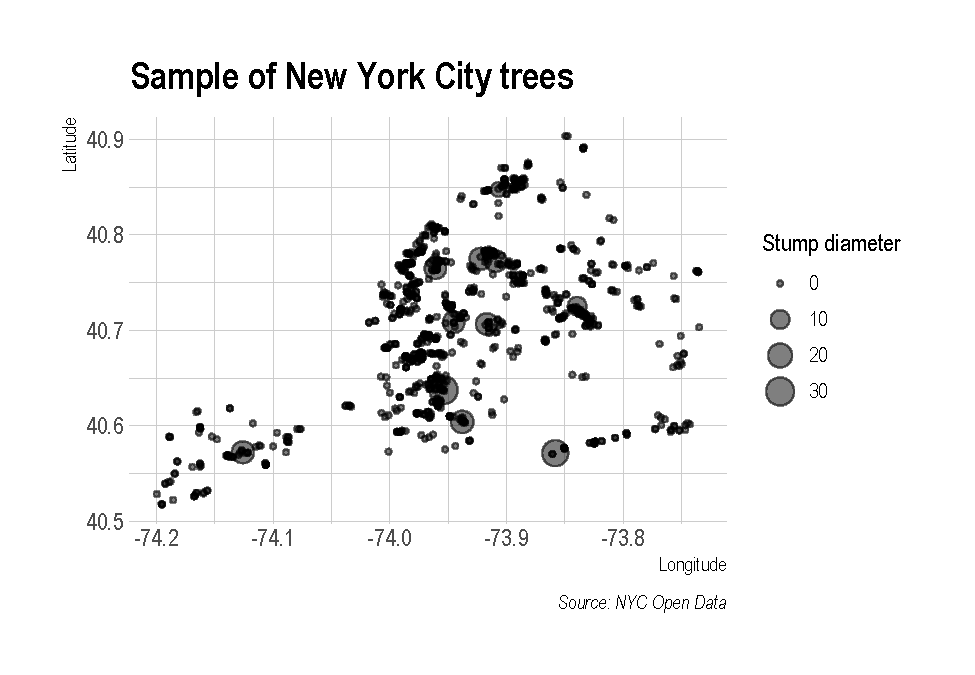
\includegraphics{07-web-apis_files/figure-latex/nyc3-1.pdf}

Not too bad. This would probably be more fun / impressive with an actual
map of New York behind it. We'll save that for the spatial lecture
that's coming up later in the course, though.

Again, I want to remind you that our first application didn't require
prior registration on the Open Data NYC website, or creation of an API
key. This is atypical. Most API interfaces will only let you access and
download data after you have registered an API key with them. This is
especially true if you want to access an API linked to a federal agency
or institution (Census, BEA, etc.). So let's work through an application
where an API key is required\ldots{}

\hypertarget{application-2-fred-data}{%
\subsection{Application 2: FRED data}\label{application-2-fred-data}}

Our second application will involve downloading data from the
\href{https://research.stlouisfed.org/docs/api/fred/}{\textbf{FRED
API}}. You will need to
\href{https://research.stlouisfed.org/useraccount/apikey}{register an
API key} if you want to follow along with my steps, so please do so
first before continuing.

As nearly every economist could tell you,
\href{https://fred.stlouisfed.org/}{FRED} is a database maintained by
the Federal Reserve Bank of St Louis. You know, the one that let's you
plot cool interactive charts
\href{https://fred.stlouisfed.org/series/GNPCA\#0}{like this one} of US
GNP since 1929.

\begin{verbatim}
## Sorry, this interactive chart is only available in the the HTML version of the notes.
\end{verbatim}

For this second example application, I'm going to show you how to
download the data underlying the above chart using the FRED API. In
fact, I'll go one better. First, I'll show you how to download it
yourself, so that you get an understanding of what's happening
underneath the hood. Then, I'll direct you to a package that does all of
the API work for you.

\hypertarget{do-it-yourself}{%
\subsubsection{Do it yourself}\label{do-it-yourself}}

As with all APIs, a good place to start is the
\href{https://research.stlouisfed.org/docs/api/fred/}{FRED API developer
docs}. If you read through these, you'd see that the endpoint path we're
interested in is
\href{https://research.stlouisfed.org/docs/api/fred/series_observations.html}{\textbf{series/observations}}.
This endpoint ``gets the observations or data values for an economic
data series''. The endpoint documentation gives a more in-depth
discussion, including the various parameters that it accepts.\footnote{Think
  of API \emph{parameters} the same way that you think about function
  \emph{arguments}. They are valid inputs (instructions) that modify the
  response to an API request.} However, the parameters that we'll be
focused on here are simply:

\begin{itemize}
\tightlist
\item
  \textbf{file\_type:} ``json'' (Not required, but our preferred type of
  output.)
\item
  \textbf{series\_id:} ``GNPCA'' (Required. The data series that we
  want.)
\item
  \textbf{api\_key:} ``YOUR\_API\_KEY'' (Required. Go and fetch/copy
  your key now.)
\end{itemize}

Let's combine these parameters with the endpoint path to view the data
directly in our browser. Head over to
\href{https://api.stlouisfed.org/fred/series/observations?series_id=GNPCA\&api_key=YOUR_API_KEY\&file_type=json}{https://api.stlouisfed.org/fred/series/observations?series\_id=GNPCA\&api\_key=YOUR\_API\_KEY\&file\_type=json},
replacing ``YOUR\_API\_KEY'' with your actual key. You should see
something like the following:

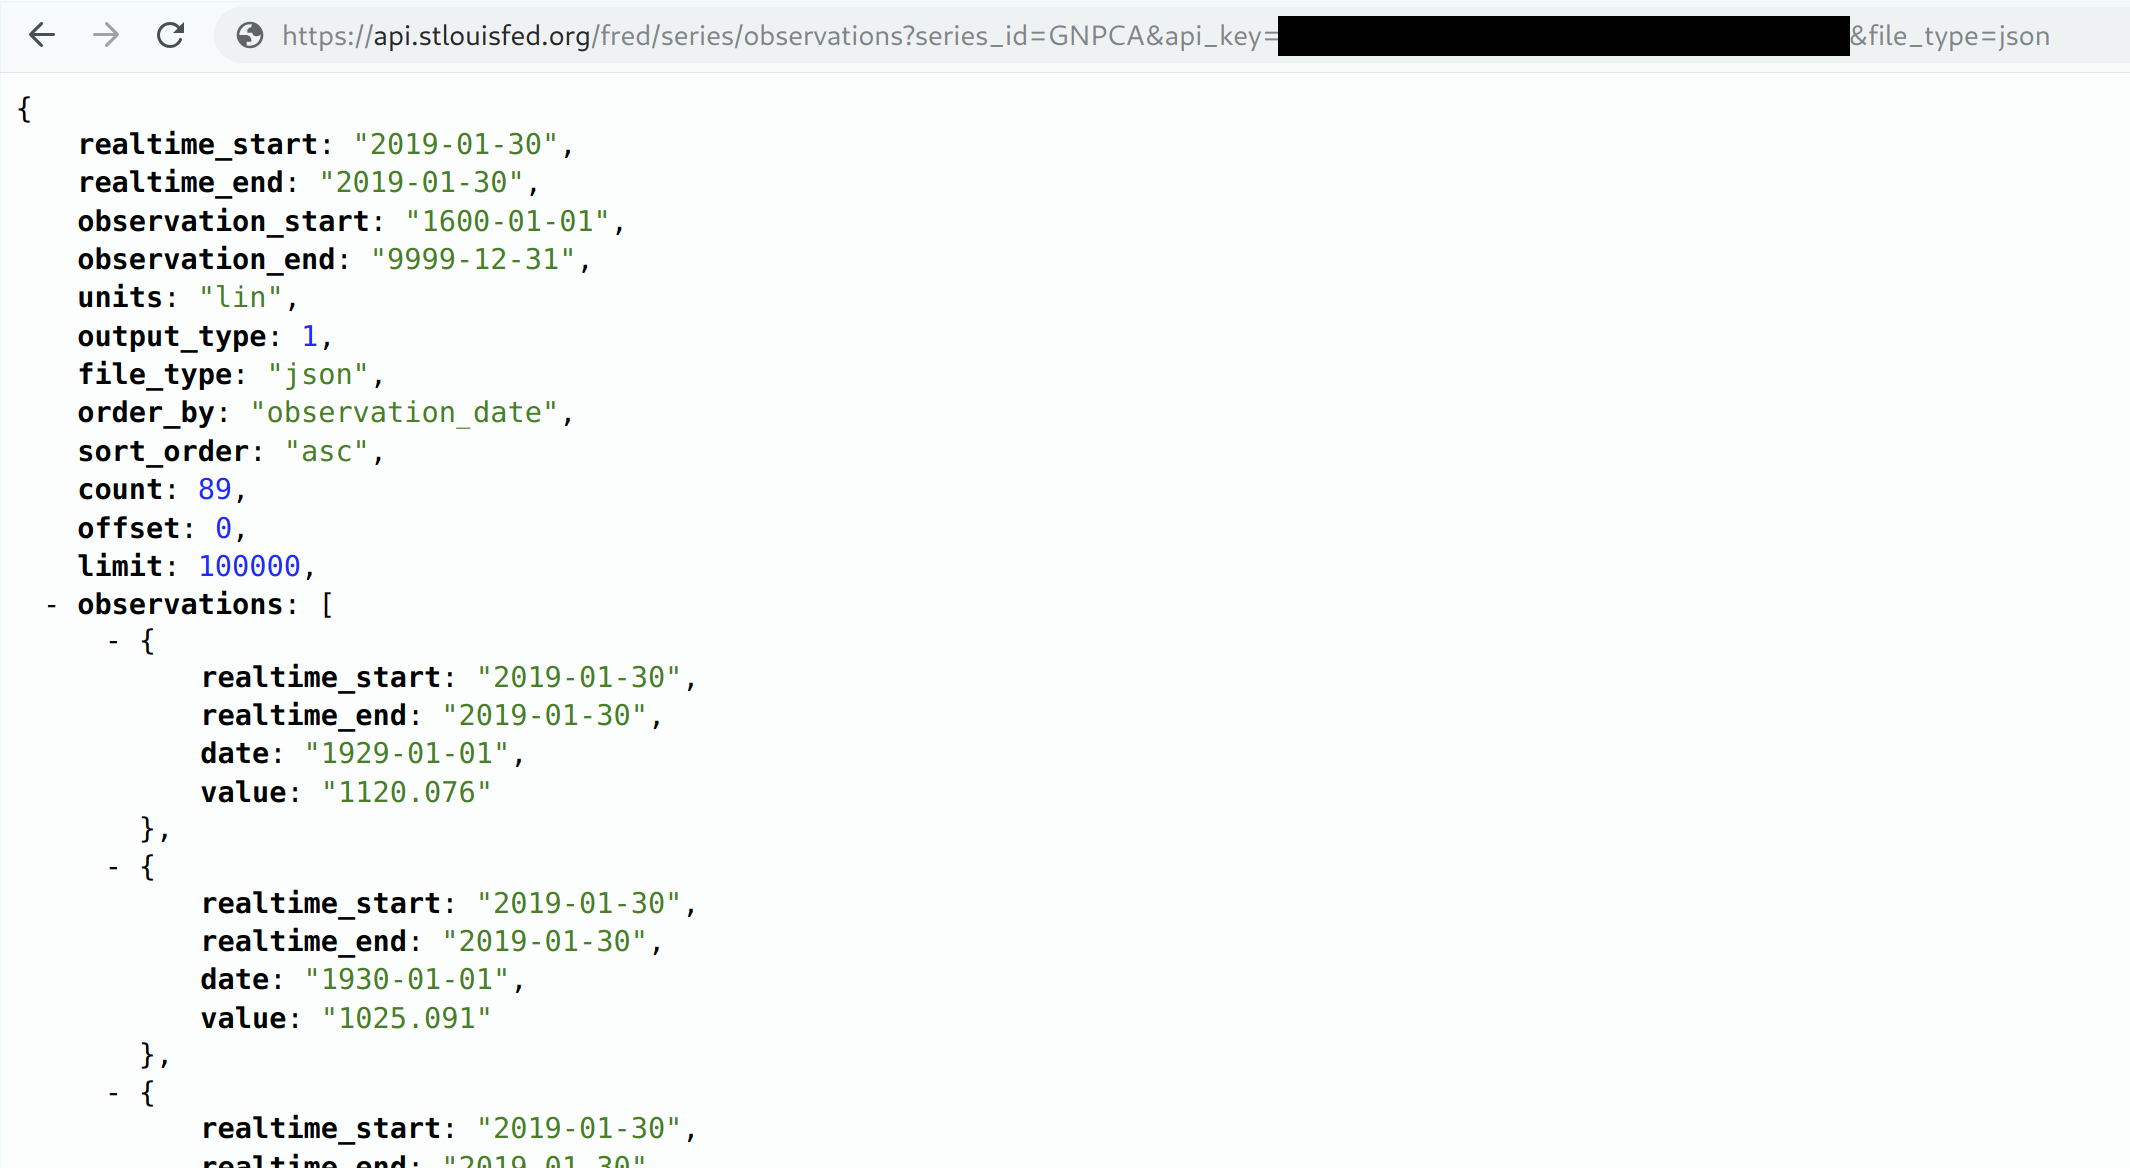
\includegraphics{pics/fred-redacted.png}

At this point you're probably tempted to read the JSON object directly
into your R environment using the \texttt{jsonlite::readJSON()}
function. And this will work. However, that's not what we're going to
here. Rather, we're going to go through the \textbf{httr} package
(\href{https://httr.r-lib.org/}{link}). Why? Well, basically because
\textbf{httr} comes with a variety of features that allow us to interact
more flexibly and securely with web APIs.

Let's start by defining some convenience variables such as the endpoint
path and the parameters (which we'll store in a list).

\begin{Shaded}
\begin{Highlighting}[]
\NormalTok{endpoint }\OtherTok{=} \StringTok{"series/observations"}
\NormalTok{params }\OtherTok{=} \FunctionTok{list}\NormalTok{(}
  \AttributeTok{api\_key=} \StringTok{"YOUR\_FRED\_KEY"}\NormalTok{, }\DocumentationTok{\#\# Change to your own key}
  \AttributeTok{file\_type=}\StringTok{"json"}\NormalTok{, }
  \AttributeTok{series\_id=}\StringTok{"GNPCA"}
\NormalTok{  )}
\end{Highlighting}
\end{Shaded}

Next, we'll use the \texttt{httr::GET()} function to request
(i.e.~download) the data. I'll assign this to an object called
\texttt{fred}.

\begin{Shaded}
\begin{Highlighting}[]
\CommentTok{\# library(httr) \#\# Already loaded above}

\NormalTok{fred }\OtherTok{=} 
\NormalTok{  httr}\SpecialCharTok{::}\FunctionTok{GET}\NormalTok{(}
    \AttributeTok{url =} \StringTok{"https://api.stlouisfed.org/"}\NormalTok{, }\DocumentationTok{\#\# Base URL}
    \AttributeTok{path =} \FunctionTok{paste0}\NormalTok{(}\StringTok{"fred/"}\NormalTok{, endpoint),    }\DocumentationTok{\#\# The API endpoint}
    \AttributeTok{query =}\NormalTok{ params                       }\DocumentationTok{\#\# Our parameter list}
\NormalTok{    )}
\end{Highlighting}
\end{Shaded}

Take a second to print the \texttt{fred} object in your console. What
you'll see is pretty cool; i.e.~it's the actual API response, including
the \emph{Status Code} and \emph{Content}. Something like:

\begin{verbatim}
## Response [https://api.stlouisfed.org/fred/series/observations?api_key=YOUR_API_KEY&file_type=json&series_id=GNPCA]
##   Date: 2019-02-01 00:06
##   Status: 200
##   Content-Type: application/json; charset=UTF-8
##   Size: 9.09 kB
\end{verbatim}

To actually extract the content (i.e.~data) from of this response, I'll
use the \texttt{httr::content()} function. Moreover, since we know that
this content is a JSON array, we can again convert it into an R object
using \texttt{jsonlite::fromJSON()}.

\begin{Shaded}
\begin{Highlighting}[]
\NormalTok{fred }\OtherTok{=} 
\NormalTok{  fred }\SpecialCharTok{\%\textgreater{}\%} 
\NormalTok{  httr}\SpecialCharTok{::}\FunctionTok{content}\NormalTok{(}\StringTok{"text"}\NormalTok{) }\SpecialCharTok{\%\textgreater{}\%} \DocumentationTok{\#\# Extract the reponse content (i.e. text)}
\NormalTok{  jsonlite}\SpecialCharTok{::}\FunctionTok{fromJSON}\NormalTok{()      }\DocumentationTok{\#\# Convert from JSON to R object}

\DocumentationTok{\#\# What type of object did we get?}
\FunctionTok{typeof}\NormalTok{(fred)}
\end{Highlighting}
\end{Shaded}

\begin{verbatim}
## [1] "list"
\end{verbatim}

It turns that the previous step has yielded a list object in
R.\footnote{complex nested lists are the law of the land when it comes
  to json information. don't worry too much about this now; just rest
  assured that r is well suited to handling these kinds of objects. it's
  one reason why r and json play so well together. we'll see more
  examples later in the course when we start working with programming
  and spatial data.} so now we need to inspect this list to better
understand its structure before extracting the information that we care
about (and coerce it to a data frame.) I'd use the base \texttt{View()}
function to do this in an interactive r session. but that won't work as
well for these lecture notes. Instead, I'll use the
\texttt{listviewer::jsonedit()} function to create an interactive widget
that renders nicely in knitted r markdown documents.

\begin{Shaded}
\begin{Highlighting}[]
\CommentTok{\# View(fred) \#\# What I\textquotesingle{}d use in an interactive R session}

\DocumentationTok{\#\# library(listviewer)        \#\# Already loaded}
\FunctionTok{jsonedit}\NormalTok{(fred, }\AttributeTok{mode =} \StringTok{"view"}\NormalTok{) }\DocumentationTok{\#\# Better for RMarkdown documents}
\end{Highlighting}
\end{Shaded}

\begin{verbatim}
## PhantomJS not found. You can install it with webshot::install_phantomjs(). If it is installed, please make sure the phantomjs executable can be found via the PATH variable.
\end{verbatim}

Luckily, this particular list object isn't too complicated. We can see
that what we're really interested in, is the \texttt{fred\$observations}
sub-element. I'll use \texttt{purrr::pluck()} to extract this element
(there are various other ways to do this) and then coerce it to a
tibble.

\begin{Shaded}
\begin{Highlighting}[]
\NormalTok{fred }\OtherTok{=}
\NormalTok{  fred }\SpecialCharTok{\%\textgreater{}\%} 
\NormalTok{  purrr}\SpecialCharTok{::}\FunctionTok{pluck}\NormalTok{(}\StringTok{"observations"}\NormalTok{) }\SpecialCharTok{\%\textgreater{}\%} \DocumentationTok{\#\# Extract the "$observations" list element}
  \CommentTok{\# .$observations \%\textgreater{}\% \#\# I could also have used this}
  \CommentTok{\# magrittr::extract("observations") \%\textgreater{}\% \#\# Or this}
  \FunctionTok{as\_tibble}\NormalTok{() }\DocumentationTok{\#\# Just for nice formatting}
\NormalTok{fred}
\end{Highlighting}
\end{Shaded}

\begin{verbatim}
## # A tibble: 94 x 4
##    realtime_start realtime_end date       value   
##    <chr>          <chr>        <chr>      <chr>   
##  1 2023-09-20     2023-09-20   1929-01-01 1120.718
##  2 2023-09-20     2023-09-20   1930-01-01 1025.678
##  3 2023-09-20     2023-09-20   1931-01-01 958.927 
##  4 2023-09-20     2023-09-20   1932-01-01 834.769 
##  5 2023-09-20     2023-09-20   1933-01-01 823.628 
##  6 2023-09-20     2023-09-20   1934-01-01 911.541 
##  7 2023-09-20     2023-09-20   1935-01-01 993.105 
##  8 2023-09-20     2023-09-20   1936-01-01 1119.585
##  9 2023-09-20     2023-09-20   1937-01-01 1178.246
## 10 2023-09-20     2023-09-20   1938-01-01 1139.642
## # ... with 84 more rows
\end{verbatim}

Okay! We've finally got our data and are nearly ready for some plotting.
Recall that \texttt{jsonlite::fromJSON()} automatically converts
everything to characters, so I'll quickly change some variables to dates
(using \texttt{lubridate::ymd()}) and numeric.

\begin{Shaded}
\begin{Highlighting}[]
\CommentTok{\# library(lubridate) \#\# Already loaded above}

\NormalTok{fred }\OtherTok{=}
\NormalTok{  fred }\SpecialCharTok{\%\textgreater{}\%}
  \FunctionTok{mutate}\NormalTok{(}\FunctionTok{across}\NormalTok{(realtime\_start}\SpecialCharTok{:}\NormalTok{date, ymd)) }\SpecialCharTok{\%\textgreater{}\%}
  \FunctionTok{mutate}\NormalTok{(}\AttributeTok{value =} \FunctionTok{as.numeric}\NormalTok{(value)) }
\end{Highlighting}
\end{Shaded}

Let's plot this sucker.

\begin{Shaded}
\begin{Highlighting}[]
\NormalTok{fred }\SpecialCharTok{\%\textgreater{}\%}
  \FunctionTok{ggplot}\NormalTok{(}\FunctionTok{aes}\NormalTok{(date, value)) }\SpecialCharTok{+}
  \FunctionTok{geom\_line}\NormalTok{() }\SpecialCharTok{+}
  \FunctionTok{scale\_y\_continuous}\NormalTok{(}\AttributeTok{labels =}\NormalTok{ scales}\SpecialCharTok{::}\NormalTok{comma) }\SpecialCharTok{+}
  \FunctionTok{labs}\NormalTok{(}
    \AttributeTok{x=}\StringTok{"Date"}\NormalTok{, }\AttributeTok{y=}\StringTok{"2012 USD (Billions)"}\NormalTok{,}
    \AttributeTok{title=}\StringTok{"US Real Gross National Product"}\NormalTok{, }\AttributeTok{caption=}\StringTok{"Source: FRED"}
\NormalTok{    )}
\end{Highlighting}
\end{Shaded}

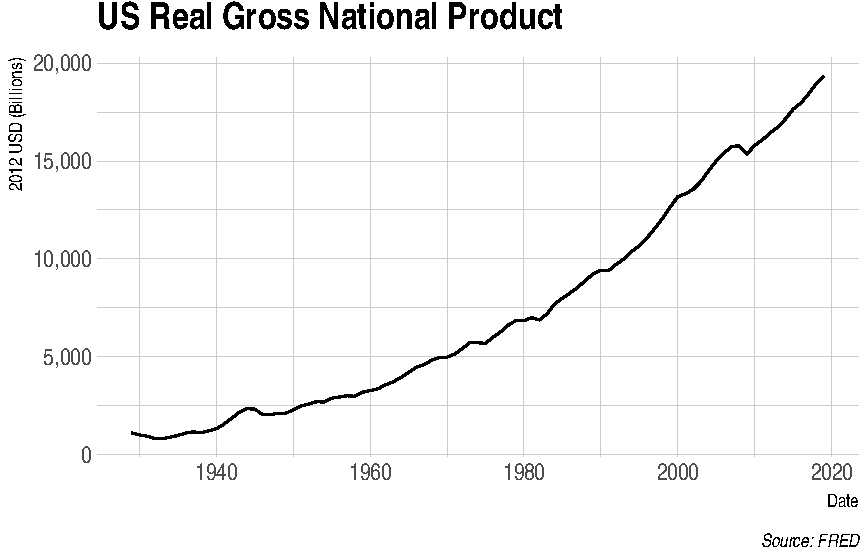
\includegraphics{07-web-apis_files/figure-latex/fred6-1.pdf}

\hypertarget{aside-safely-store-and-use-api-keys-as-environment-variables}{%
\subsubsection{Aside: Safely store and use API keys as environment
variables}\label{aside-safely-store-and-use-api-keys-as-environment-variables}}

In the above example, I assumed that you would just replace the
``YOUR\_FRED\_KEY'' holder text with your actual API key. This is
obviously not very secure or scalable, since it means that you can't
share your R script without giving away your key.\footnote{The same is
  true for compiled R Markdown documents like these lecture notes.}
Luckily, there's an easy way to safely store and use sensitive
information like API keys or passwords: Simply save them as an R
\href{https://stat.ethz.ch/R-manual/R-devel/library/base/html/EnvVar.html}{\textbf{environment
variables}}. There are two, closely related approaches:

\begin{enumerate}
\def\labelenumi{\arabic{enumi}.}
\tightlist
\item
  Set an environment variable for the current R session only.
\item
  Set an environment variable that persists across R sessions.
\end{enumerate}

Let's briefly review each in turn.

\hypertarget{set-an-environment-variable-for-the-current-r-session-only}{%
\paragraph{1) Set an environment variable for the current R session
only}\label{set-an-environment-variable-for-the-current-r-session-only}}

Defining an environment variable for the current R session is very
straightforward. Simply use the base \texttt{Sys.setenv()} function. For
example:

\begin{Shaded}
\begin{Highlighting}[]
\DocumentationTok{\#\# Set new environment variable called MY\_API\_KEY. Current session only.}
\FunctionTok{Sys.setenv}\NormalTok{(}\AttributeTok{MY\_API\_KEY=}\StringTok{"abcdefghijklmnopqrstuvwxyz0123456789"}\NormalTok{) }
\end{Highlighting}
\end{Shaded}

Once this is done, you can then safely assign your key to an object ---
including within an R Markdown document that you're going to knit and
share --- using the \texttt{Sys.getenv()} function. For example:

\begin{Shaded}
\begin{Highlighting}[]
\DocumentationTok{\#\# Assign the environment variable to an R object}
\NormalTok{my\_api\_key }\OtherTok{=} \FunctionTok{Sys.getenv}\NormalTok{(}\StringTok{"MY\_API\_KEY"}\NormalTok{)}
\DocumentationTok{\#\# Print it out just to show that it worked}
\NormalTok{my\_api\_key}
\end{Highlighting}
\end{Shaded}

\begin{verbatim}
## [1] "abcdefghijklmnopqrstuvwxyz0123456789"
\end{verbatim}

\textbf{Important:} While this approach is very simple, note that in
practice the \texttt{Sys.setenv()} part should only be run directly in
your R console. \emph{Never} include code chunks with sensitive
\texttt{Sys.setenv()} calls in an R Markdown file or other shared
documents.\footnote{Since the new R environment variable is defined for
  the duration of the current session, R Markdown will have access to
  this variable irrespective of whether it was defined in the R Markdown
  script or not.} That would entirely defeat the purpose! Apart from the
annoyance of having to manually set my API key each time I start a new R
session, this is one reason that I prefer the next approach of
persisting environment variables across sessions\ldots{}

\hypertarget{set-an-environment-variable-that-persist-across-r-sessions}{%
\paragraph{2) Set an environment variable that persist across R
sessions}\label{set-an-environment-variable-that-persist-across-r-sessions}}

The trick to setting an R environment variable that is available across
sessions is to add it to a special file called
\texttt{\textasciitilde{}/.Renviron}. This is a text file that lives on
your home directory --- note the \texttt{\textasciitilde{}/} path ---
which R automatically reads upon startup. Because
\texttt{\textasciitilde{}/.Renviron} is just a text file, you can edit
it with whatever is your preferred text editor. However, you may need to
create it first if it doesn't exist. A convenient way to do all of this
from RStudio is with the \texttt{usethis::edit\_r\_environ()} function.
You will need to run the next few lines interactively:

\begin{Shaded}
\begin{Highlighting}[]
\DocumentationTok{\#\# Open your .Renviron file. Here we can add API keys that persist across R sessions.}
\NormalTok{usethis}\SpecialCharTok{::}\FunctionTok{edit\_r\_environ}\NormalTok{() }
\end{Highlighting}
\end{Shaded}

This will open up your \texttt{\textasciitilde{}/.Renviron} file in a
new RStudio window, which you can then modify as needed. As an example,
let's say that you want to add your FRED API key as an environment
variable that persists across sessions. You can do this by simply adding
a line like the below to your \texttt{\textasciitilde{}/.Renviron} file
and saving.\footnote{I suggest calling it something that's easy to
  remember like ``FRED\_API\_KEY'', but as you wish.}

\begin{verbatim}
FRED_API_KEY="abcdefghijklmnopqrstuvwxyz0123456789" ## Replace with your actual key
\end{verbatim}

Once you have saved your changes, you'll need to refresh so that this
new environment variable is available in the current session. You could
also restart R, but that's overkill.

\begin{Shaded}
\begin{Highlighting}[]
\DocumentationTok{\#\# Optional: Refresh your .Renviron file.  }
\FunctionTok{readRenviron}\NormalTok{(}\StringTok{"\textasciitilde{}/.Renviron"}\NormalTok{) }\DocumentationTok{\#\# Only necessary if you are reading in a newly added R environment variable}
\end{Highlighting}
\end{Shaded}

\textbf{Challenge:} Once you've refreshed your
\texttt{\textasciitilde{}/.Renviron} file, try to re-download the FRED
data from earlier. This time call your FRED API key directly as an
environment variable in your parameter list using \texttt{Sys.getenv()}
like this:

\begin{Shaded}
\begin{Highlighting}[]
\NormalTok{params }\OtherTok{=} \FunctionTok{list}\NormalTok{(}
  \AttributeTok{api\_key=} \FunctionTok{Sys.getenv}\NormalTok{(}\StringTok{"FRED\_API\_KEY"}\NormalTok{), }\DocumentationTok{\#\# Get API directly and safely from the stored environment variable}
  \AttributeTok{file\_type=}\StringTok{"json"}\NormalTok{, }
  \AttributeTok{series\_id=}\StringTok{"GNPCA"}
\NormalTok{  )}
\end{Highlighting}
\end{Shaded}

We're going to be revisiting (and setting) environment variables once we
get to the cloud computation part of the course. So please make sure
that you've understood this section and that your new FRED API key
works.

\hypertarget{use-a-package}{%
\subsubsection{Use a package}\label{use-a-package}}

One of the great features about the R (and data science community in
general) is that someone has probably written a package that does all
the heavy API lifting for you. We'll come across many examples during
the remainder of this course, but for the moment I want to flag the
\textbf{fredr} package
(\href{http://sboysel.github.io/fredr/index.html}{link}). Take a look at
the ``Get started'' page to see how you could access the same GDP data
as above, but this time going through a package.

\hypertarget{summary}{%
\subsection{Summary}\label{summary}}

\begin{itemize}
\tightlist
\item
  An API is a set of rules and methods that allow one computer or
  program (e.g.~host server) to talk to another (e.g.~client or
  browser).
\item
  We can access information through an API directly by specifying a
  valid API endpoint.

  \begin{itemize}
  \tightlist
  \item
    The API endpoint for most web-based applications will be a URL with
    either JSON or XML content.
  \end{itemize}
\item
  Some APIs don't require an access key or token, but most do. You can
  add this key as a parameter to the API endpoint.
\item
  Downloading content from an API endpoint to our local computer (i.e.~R
  environment) can be done in a variety of ways.

  \begin{itemize}
  \tightlist
  \item
    E.g. \texttt{jsonlite::readJSON()} to read the the JSON array
    directly, or \texttt{httr::GET()} to download the entire response,
    or installing a package that does the job for us.
  \end{itemize}
\item
  \textbf{Next lecture:} Regression analysis in R. (The start of the
  analysis and programming section of the course.)
\end{itemize}

\hypertarget{further-resources-and-exercises}{%
\subsection{Further resources and
exercises}\label{further-resources-and-exercises}}

\begin{itemize}
\item
  \href{https://www.pscp.tv/w/1ynKOpVnERrGR}{Here} is a short, live
  video stream that I did for scraping traffic fatality data from
  \href{https://data.lacity.org/}{LA's Open Data portal}. As I mention
  in the video, this covers very similar ground to today's lecture. But
  I do expand a bit on using API parameters to query (i.e.~wrangle and
  summarise) data directly up on the host server before scraping it.
\item
  \href{https://twitter.com/tclavl}{Tyler Clavelle} has written several
  cool \href{https://tclavelle.github.io/blog/}{blog posts} on
  interacting with APIs through R. I especially recommend going over ---
  and replicating --- his excellent
  \href{https://tclavelle.github.io/blog/r_and_apis/}{tutorial on the
  GitHub API}.
\item
  Jonathan Regenstein has a nice post on RStudio's \emph{R Views} blog,
  ``\href{https://rviews.rstudio.com/2018/09/12/gdp-via-api/}{GDP Data
  via API}'', which treads a similar path to my FRED example. Except he
  uses the Bureau of Economic Analysis (BEA) API.
\item
  Greg Reda's
  ``\href{http://www.gregreda.com/2015/02/15/web-scraping-finding-the-api/}{Web
  Scraping 201: finding the API}'' covers much of the same ground as we
  have here. While he focuses on Python tools, I've found it to be a
  handy reference over the years. (You can also take a look at the
  earlier posts in Greg's webscraping series ---
  \href{http://www.gregreda.com/2013/03/03/web-scraping-101-with-python/}{Part
  1} and
  \href{http://www.gregreda.com/2013/04/29/more-web-scraping-with-python/}{Part
  2} --- to see some Python equivalents of the \texttt{rvest} tools that
  we've been using.)
\item
  Ian London (another Python user) has a nice blog post on
  ``\href{https://ianlondon.github.io/blog/web-scraping-discovering-hidden-apis/}{Discovering
  hidden APIs}'' from Airbnb.
\item
  Finally, while the methods covered in the last two lectures should
  have you covered for 95\% (99\%?) of your webscraping needs, there are
  some corner cases where they won't work. In particular, you may run
  into cases where website content is rendered dynamically with
  JavaScript. In times like these, you'll need to spin up a so-called
  ``headless'' browser to extract the content. More
  \href{https://rud.is/b/2017/02/09/diving-into-dynamic-website-content-with-splashr/}{here}
  and
  \href{https://twitter.com/grant_mcdermott/status/1192889722672041984}{here}.
\end{itemize}

\end{document}
